\documentclass[12pt]{article}
 
\usepackage{amsmath,amsthm,amssymb}
\usepackage{graphicx} 
\graphicspath{{./images/}}
\begin{document}
 
%\renewcommand{\qedsymbol}{\filledbox}
 
\title{Homework 8}
\author{Rafael Betita\\ 
MATH 005BH - Single Variable Calculus II}
 
\maketitle
 
\newpage
\section{7.5 Techniques of Integration} 1-53 EOO

\begin{enumerate}
  \item $\int\frac{\cos{x}}{1-\sin{x}}dx$
        \begin{align*}
            u &= 1-\sin{x}\\\\
            (-1)du &= \cos{x} dx\\\\
            &=-\int\frac{du}{1-u}\\\\
            &=-ln|1-\sin{x}|+C
        \end{align*}
    \addtocounter{enumi}{3}\item $\int \frac{t}{t^4+2}dt$
        \begin{align*}
            &= \int \frac{t}{(t^2)^2+2}dt & u &= t^2 & \frac{1}{2}du &= tdt\\\\
            &= \frac{1}{2}\int \frac{du}{u^2+2} && \text{Use tangent identity here}\\\\
            &= \frac{1}{2}\left[\left(\frac{1}{\sqrt{2}}\right)\tan^{-1}\left(\frac{t^2}{\sqrt{2}}\right)\right] +C\\\\
            &= \frac{1}{2\sqrt{2}}\left[\tan^{-1}\left(\frac{t^2}{\sqrt{2}}\right)\right] + C \\
        \end{align*}
    \addtocounter{enumi}{3}\item $\int_{2}^{4}\frac{x+2}{x^2+3x-4}dx$
        \begin{align*}
             \int_{2}^{4}\frac{x+2}{(x+4)(x-1)}dx = \frac{A}{(x+4)}+\frac{B}{(x-1)}\\\\
             x+2 = A(x-1) + B(x+4)\\
             x(4) \xrightarrow{} -4+2=A(-5)+B(0) \xrightarrow{} A=\frac{2}{5}\\
             x(1) \xrightarrow{} 1+2= A(0)+B(5) \xrightarrow{} B=\frac{3}{5}\\\\
             \int_{2}^{4}\frac{x+2}{(x+4)(x-1)}dx = \int_{2}^{4}\frac{\frac{2}{5}}{(x+4)}dx+\int_{2}^{4}\frac{\frac{3}{5}}{(x-1)}dx\\\\
             \frac{2}{5}\ln{\Big|x+4\Big|}_2^4+\frac{3}{5}\ln{
             \Big|x-1\Big|}_2^4\\\\
             \left(\frac{2}{5}\ln{8} - \frac{2}{5}\ln{6}\right) + \left(\frac{3}{5}\ln{3}-0\right) 
         \end{align*}
    \addtocounter{enumi}{3}\item $\int\sin^5{t}\cos^4t$
        \begin{align*}
            &=\int (\sin^2t)^2(\cos^2t)^2\sin{t}dt \\
            &= -\int (1-u^2)^2(u^2)^2du &u &= \cos{t} &-du &= \sin{t}\\
            &=-\int (1-2u^2+u^4)(u^4)du \\
            &=-\int (u^4-2u^6+u^8)du \\
            &=-\frac{\cos^5t}{5}+\frac{2\cos^7t}{7}-\frac{cos^9t}{9}+C
        \end{align*}
    
    \newpage\addtocounter{enumi}{3}\item $\int_0^\pi t\cos^2tdt$
        \begin{align*}
            &\int_0^\pi \left(\frac{1}{2}t + \frac{1}{2}t\cos2t\right)dt\\\\
            &\left[\frac{t^2}{4}\right]_0^\pi + \frac{1}{2}\int_0^\pi t\cos2tdt          & u &= t  & dv &= \cos2tdt \\\\
            &\frac{\pi^2}{4}+\frac{1}{2}\left[\frac{1}{2}t\sin2t\right]_0^\pi-\frac{1}{2}\int_0^\pi\frac{1}{2}\sin2tdt & du &=dt &v&=\frac{1}{2}\sin{2t}\\\\
            &\frac{\pi^2}{4}+[0] +\frac{1}{8}\left\bigg[\cos2t\right\bigg]_0^\pi = \frac{\pi^2}{4}
        \end{align*}
    \addtocounter{enumi}{3}\item \int$\arctan\sqrt{x}\ dx$
        \begin{align*}
            & u = \sqrt{x} & u^2 = x & &2udu=dx 
        \end{align*}
        \begin{align*}
        2\int u\arctan u \ du 
        \end{align*}
        \begin{tabular}{c|c}
            D & I\\ \hline 
            +\arctan u & $u$\\ \hline
            -$\frac{1}{1+u^2}$ & $\frac{u^2}{2}$\\
        \end{tabular}
        \quad \quad \quad \quad \quad $2\left[\frac{u^2\arctan{u}}{2}\right]-2\int\frac{u^2}{2+2u^2}du$
        \begin{align*}
            &= x\arctan\sqrt{x}-\int \left[1-\frac{1}{1+u^2}\right]du\\\\
            &= x\arctan{\sqrt{x}}-\sqrt{x}+\arctan{\sqrt{x}} + C\\\\
            &= (x+1)\arctan{\sqrt x}-\sqrt{x} + C
        \end{align*} \newpage
    \addtocounter{enumi}{3}\item $\int_0^1\frac{1+12t}{1+3t}dt$
        \begin{align*}
            \int_0^1 \left(\frac{(12t+4)-3}{3t+1}\right) &= \int_0^1 \left(\frac{4(3t+1)-3}{3t+1}\right) = \int_0^14dt - \int_0^1\frac{3}{3t+1}\\\\
            4t\bigg|_0^1-\ln|3t+1|\bigg|_0^1 &= 4-0 - (\ln4 - 0) \\
            &= 4 - \4ln4
         \end{align*}
    \addtocounter{enumi}{3}\item $\int\ln\left(x+\sqrt{x^2-1}\right)dx$
        \begin{align*}
            u&= \ln{(x+\sqrt{x^2-1})} & dv &= dx \\
            du&= \frac{1}{x+\sqrt{x^2-1}}\left(1+\frac{2x}{2\sqrt{x^2-1}}\right)dx & v &= x\\
            du&=\frac{1}{x+\sqrt{x^2-1}}\left(\frac{\sqrt{x^2+1}+x}{\sqrt{x^2-1}}\right)dx\\
            du&= \frac{1}{\sqrt{x^2-1}}dx\\
            &=x\ln{(x+\sqrt{x^2-1})}-\int\frac{x}{\sqrt{x^2-1}}\\
            &=x\ln{(x+\sqrt{x^2-1})}-\sqrt{x^2-1} + C
        \end{align*}
    \addtocounter{enumi}{3}\item $\int\sqrt{3-2x-x^2}dx$
        \begin{align*}
            \int\sqrt{(3+1)-(x^2+2x+1)}dx &= \int\sqrt{4-(x+1)^2}dx \\
            &= \int\sqrt{4-4sin^2\theta}(2\cos\theta) d\theta\\
            4\int\cos^2\theta d\theta = \frac{4}{2}\int(1+\cos2\theta)d\theta &= 2\theta + \frac{2}{2}\sin{2\theta}+C\\
            2\arcsin{\left(\frac{x+1}{2}\right)}&+\frac{(x+1)(\sqrt{4-(x+1)^2})}{2} + C
        \end{align*} \newpage
    \addtocounter{enumi}{3}\item $\int^\frac{\pi}{4}_0\tan^3\theta sec^2\theta d\theta$
        \begin{align*}
            u = \tan{\theta}, du = \sec^2\theta d \theta\\
            \int^\frac{\pi}{4}_0 u^3du = \left[\frac{u^4}{4}\right]_0^\pi = \frac{1}{4}
        \end{align*}
    \addtocounter{enumi}{3}\item $\int\theta \tan^2\theta \ d\theta$
        \begin{align*}
            &\int\theta(\sec^2\theta-1) d\theta\\
            u &= \theta  &dv =(\sec^2\theta-1)\\
            du &= d\theta &v =(\tan\theta-\theta)\\
            &=\theta\tan\theta-\theta^2-\int (\tan\theta-\theta)d\theta \\
            &= \theta\tan\theta-\theta^2-\ln{|\sec{\theta}|}+\frac{\theta^2}{2} \\
            &= \theta\tan\theta-\frac{\theta^2}{2}-\ln{|\sec{\theta}|}+C             
        \end{align*}
    \addtocounter{enumi}{3}\item $\int x^5 \ e^{-x^3}dx$
        \begin{align*}
            u &= -x^3 &-\frac{1}{3}du &= x^2dx\\
            \int x^3x^2e^udx = \frac{1}{3}\int u\cdot e^u du\\
            \alpha &= u &d\beta &= e^u\\
            d\alpha &= 1 &\beta &= e^u\\
            =\frac{1}{3}\left[(-x^3)e^{-x^3} - e^{-x^3}\right] + C\\
            =-\frac{1}{3}\left[e^{-x^3}(x^3+1)\right] + C\\
        \end{align*}\newpage
    \addtocounter{enumi}{3}\item $\int\frac{1}{x\sqrt{4x+1}}dx$
        \begin{align*}
            &u = \sqrt{4x+1} & u^2=4x+1 && \frac{1}{2}udu=dx &&x=\frac{u^2-1}{4}
        \end{align*}
        \begin{align*}
            \frac{1}{2}\int\frac{u}{(x)u}du = \frac{1}{2}\int\frac{4}{u^2-1}du
        \end{align*}
        \begin{align*}
            A(u+1)+B(u-1)=4 && A = 2 && B = -22 &
        \end{align*}
        \begin{align*}
            \frac{1}{2}\int\frac{2}{u-1}du-\frac{1}{2}\int\frac{2}{u+1} du\\\\
            \ln{|\sqrt{4x-1}-1|} - \ln{|\sqrt{4x-1}+1|} + C             
        \end{align*}
    \addtocounter{enumi}{3}\item $\int x^2\sinh{mx}dx$\newline\newline
        \begin{tabular}{c|c}
            D & I \\\hline
            $+x^2$  & $\sinh{mx}$\\\hline
            $-2x$ & $\frac{1}{m}\cosh{mx}$\\\hline
            $+2$ & $\frac{1}{m^2}\sinh{mx}$\\\hline
            $-0$ & $\frac{1}{m^3}\cosh{mx}$\\\hline
        \end{tabular}
        \begin{equation*}
            \frac{x^2}{m}\cosh{mx}-\frac{2x}{m^2}\sinh{mx}+\frac{2}{m^3}\cosh{mx}+C
        \end{equation*}
\end{enumerate}

\newpage
\section{7.8  Improper Integrals} 1-41 EOO

\begin{enumerate}
    \item Explain why each of the following integrals is improper
        \begin{enumerate}
            \item 
                $\int_1^2\frac{x}{x-1}dx$ 
                \\\\\textt{This is a discontinuous integral, since bound includes vertical asymptote x = 1}
            \item 
                $\int^\infty_0\frac{1}{1+x^3}dx$
                \\\\\textt{This is also a infinite integral. As x approaches infinity, the integral converges.}
            \item 
                $\int_{-\infty}^\infty x^2e^{-x^2}dx$
                \\\\\textt{This integral has an infinite bound on both ends, making it an infinite integral.}
            \item
                $\int_0^\frac{\pi}{4}\cot{x}dx$
                \\\\\textt{This is an discontinuous integral as x \xrightarrow{}0,  \ $\cot{x}$ approaches infinity}
        \end{enumerate}

    \addtocounter{enumi}{3}\item $\int^\infty_3\frac{1}{(x-2)^\frac{3}{2}}dx$
        \begin{align*}
            \lim_{t\to\infty}\int^t_3\frac{1}{(x-2)^{\frac{3}{2}}} = \lim_{t\to\infty}-2(x-2)^{-\frac{1}{2}}\bigg|_3^t = \lim_{t\to\infty}\left[-\frac{2}{\sqrt{t-2}}+\frac{2}{\sqrt{1}}\right] = 0+2= 0
        \end{align*}
    \addtocounter{enumi}{3}\item $\int^\infty_2e^{-5p}dp$    
        \begin{align*}
            \lim_{t\to\infty}\int^t_2e^{-5p}dp = \lim_{t\to\infty}\left[-\frac{1}{5}e^{-5p}\right]^t_2 = \lim_{t\to\infty}\left[-\frac{1}{5}e^{-5t}+\frac{1}{5}e^{-10}\right] = 0 + \frac{1}{5}e^{-10}
        \end{align*}\newpage
    \addtocounter{enumi}{3}\item $\int^\infty_{-\infty}xe^{-x^2}dx$
        \begin{align*}
            u = -x^2 \\ -\frac{1}{2}du = xdx\\
            -\frac{1}{2}\int^\infty_{-\infty}e^udu = -\frac{1}{2}\left[\int^\infty_{0}e^udu+\int^0_{-\infty}e^udu\right]\\\\
            = -\frac{1}{2}\left[(e^{-\infty^2}-e^{-0^2})+(e^{-0^2}-e^{-\infty^2})\right] \\\\ = -\frac{1}{2}\left[(0-1)+(1-0)\right] \\
            = \frac{1}{2} - \frac{1}{2} = 0
        \end{align*}
    \addtocounter{enumi}{3}\item $\int^\infty_1\frac{1}{x^2+x}dx$
        \begin{align*}
            \lim_{t\to\infty}\int_1^t\frac{1}{x(x+1)}dx\\
            A(x+1) + B(x) = 1; A = 1, B = -1\\\\
            \lim_{t\to\infty}\left[\int_1^t\left(\frac{1}{x}-\frac{1}{1+x}dx\right)\right]\\\\
            \lim_{t\to\infty}\left[\ln{|x|}-\ln{(|1+x|)}\right]_1^t = \lim_{t\to\infty}\left[\ln{\left|\frac{x}{1+x}\right|}\right]_1^t\\\\
            \lim_{t\to\infty}\left[\ln{\frac{t}{1+t}}-\ln{\frac{1}{1+1}}\right] = 0 - \ln{\frac{1}{2}}
        \end{align*}\newpage
    \addtocounter{enumi}{3}\item $\int^\infty_1\frac{\ln{x}}{x}dx$
        \begin{align*}
            u = \ln{x} && du = \frac{1}{x}dx
        \end{align*}
        \begin{equation*}
            \int^\infty_1 udu = \lim_{t\to\infty}\int^t_1udu = \lim_{t\to\infty}\left[\frac{u^2}{2}\right]_1^t
        \end{equation*}
        \begin{equation*}
            \lim_{t\to\infty}\left[\frac{(\ln{t})^2}{2}-\frac{1}{2}\right] = \infty
        \end{equation*}
    \addtocounter{enumi}{3}\item $\int^\infty_0e^{-\sqrt{y}}dy$
        \begin{align*}
            u = -\sqrt{y} && -2\sqrt{y}du = dy && 2udu = dy 
        \end{align*}
        \begin{tabular}{c|c}
            D & I \\\hline
            $+u$ & $e^u$\\
            $-1$ & $e^u$\\
            $+0$ & $e^u$
        \end{tabular}
        \quad\quad
        $\lim_{t\to\infty}2\int_0^te^uudu = \lim_{t\to\infty}2\left[u e^u-e^u\right]$\\
        \begin{multline*}
            \lim_{t\to\infty} \left[-2\sqrt{y}e^{-\sqrt{y}}-2e^{-\sqrt{y}}\right]_0^t = \lim_{t\to\infty} \left[-2\sqrt{t}e^{-\sqrt{t}}-2e^{-\sqrt{t}}+2\right] = 2
        \end{multline*}
        \begin{align*}
            \lim_{t\to\infty}-\frac{2\sqrt{t}}{e^{\sqrt{t}}}\overset{H}{=}\lim_{t\to\infty}-\frac{\frac{2}{2\sqrt{t}}}{\frac{1}{2\sqrt{t}}e^{\sqrt{t}}} = \lim_{t\to\infty}\frac{-2}{e^{\sqrt{t}}}=0    
        \end{align*}
    \addtocounter{enumi}{3}\item $\int^{14}_{-2}\frac{dx}{\sqrt[4]{x+2}}$    
        \begin{align*}
            \lim_{t\to -2^+}\int_t^{14}\frac{dx}{\sqrt[4]{x+2}} = \lim_{t\to -2^+}\int_t^{14}\frac{4u^3du}{u}=\lim_{t\to -2^+}4\int_t^{14}u^2du
        \end{align*}
        \begin{align*}
            u = \sqrt[4]{x+2} \to 4u^3du = dx
        \end{align*}
        \begin{align*}
            \lim_{t\to -2^+}4\left[\frac{u^3}{3}\right]_t^{14}
            =\lim_{t\to -2^+}4\left[\frac{(\sqrt[4]{x+2})^{3}}{3}\right]_t^{14}=\lim_{t\to -2^+}4\left[\frac{8}{3}-\frac{(\sqrt[4]{t+2})^3}{3}\right]= \frac{32}{3}
        \end{align*}\newpage
    \addtocounter{enumi}{3}\item $\int_0^9\frac{1}{\sqrt[3]{x-1}}dx$\
        \begin{align*}
            \lim_{t\to 1^-}\left(\int_0^t\frac{dx}{\sqrt[3]{x-1}}\right)
            +\lim_{t\to 1+}\left(\int_t^9\frac{dx}{\sqrt[3]{x-1}}\right)
        \end{align*}
        \begin{align*}
            u = \sqrt[3]{x-1} \to 3u^2du = dx
        \end{align*}
        \begin{align*}
            \lim_{t\to 1^-}\left(\int_0^t\frac{3u^2du}{u}\right) 
            =\lim_{t\to 1^-} \left[\frac{3u^2}{2}\right]_0^t
            =\lim_{t\to 1^-} \left[\frac{3(x-1)^{\frac{2}{3}}}{2}\right]_0^t 
            = -\frac{3}{2}\\
            \lim_{t\to 1^+}\left(\int_t^9\frac{3u^2du}{u}\right) 
            =\lim_{t\to 1^+} \left[\frac{3u^2}{2}\right]_t^9
            =\lim_{t\to 1^+} \left[\frac{3(x-1)^{\frac{2}{3}}}{2}\right]_t^9 
            = 6
        \end{align*}
        \begin{align*}
            6-\frac{3}{2} = \frac{12}{2}-\frac{3}{2} = \frac{9}{2}
        \end{align*}
    \addtocounter{enumi}{3}\item $\int_0^1r\ln{r}dr$
        \begin{align*}
            \lim_{t\to 0^+}\int_t^1r\ln{r}dr
        \end{align*}
        \begin{align*}
            u &= \ln{r} & dv &= rdr\\
            du &= \frac{dr}{r} & v &=\frac{r^2}{2}
        \end{align*}
        \begin{align*}
            \lim_{t\to 0^+}\left[\frac{r^2\ln{r}}{2}-\frac{1}{2}\int^1_trdr\right]^1_t 
            = \left[0-\frac{1}{4}\right]-\left[0-0\right]=-\frac{1}{4}
        \end{align*}\newpage
    \addtocounter{enumi}{3}\item $S=\{\ (x,y) \  | \ x \geq 1, 0 \leq y, \leq e^{-x}\}$
        \begin{align*}
            \int_1^\infty e^{-x}dx=\lim_{t\to\infty}\int^t_1e^{-x}dx=\lim_{t\to\infty}-e^{-x}\bigg|_1^t = \lim_{t\to\infty}\left[-e^{-t}+e^{-1}\right]=[0+e^{-1}]
        \end{align*}
\end{enumerate}
    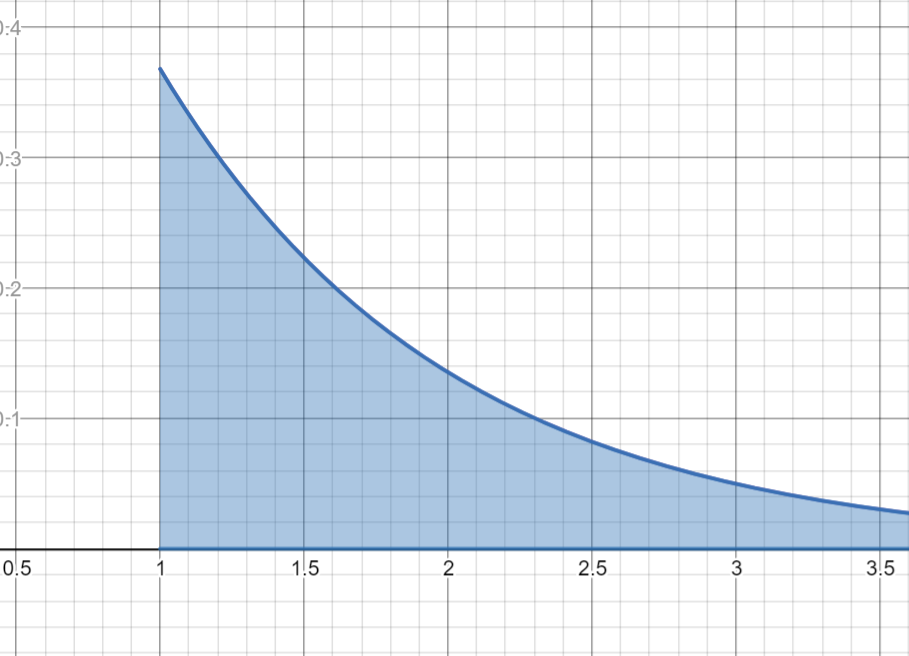
\includegraphics[width=\textwidth]{41}
 
 
\newpage
\section{More Practice with Integrals}

\begin{enumerate}
    \item $\int (1+x)(1+x^2)dx$
        \begin{align*}
             &=\int dx + \int x^2dx + \int dx + \int x^3dx \\
             &= x +\frac{x^3}{3} + \frac{x^2}{2} + \frac{x^4}{4} + C 
        \end{align*}
        
    \item $\int \frac{1+2x+2x^2}{x^2}dx$
        \begin{align*}
            &= \int \left(\frac{1}{x^2}+\frac{2}{x}+2\right)dx\\
            &= -\frac{1}{x}+2\ln|x|+2x+C
        \end{align*}

    \item $\int \frac{xdx}{9-4x^2}$
        \begin{align*}
            u &= 9-4x^2\\
            -\frac{1}{8}du &= xdx\\
            &= -\frac{1}{8}\int\frac{du}{u}\\
            &= -\frac{1}{8}\left(ln|9-4x^2|\right)+C\\
        \end{align*}
    
\end{enumerate}
\end{document}